\section{Topical\_\-DIL\_\-Files  Class Reference}
\label{classTopical__DIL__Files}\index{Topical_DIL_Files@{Topical\_\-DIL\_\-Files}}
{\tt \#include $<$dil2al.hh$>$}

Inheritance diagram for Topical\_\-DIL\_\-Files::\begin{figure}[H]
\begin{center}
\leavevmode
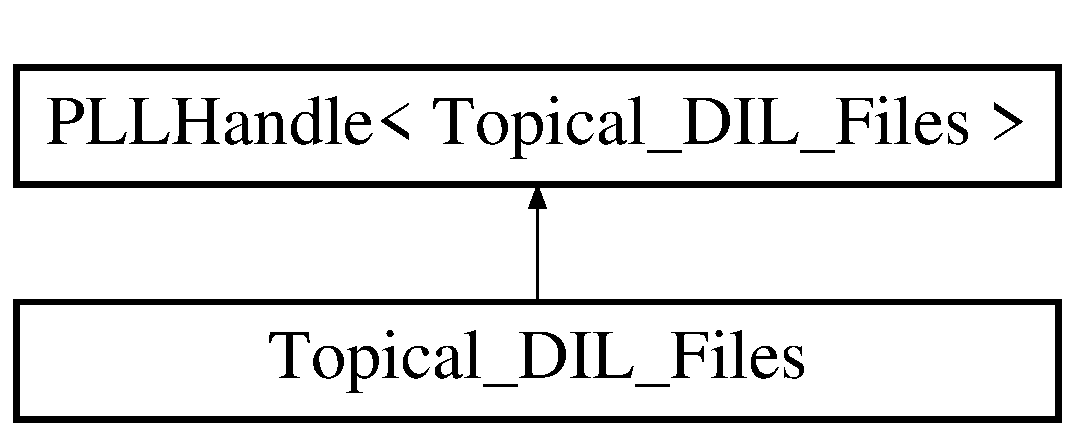
\includegraphics[height=2cm]{classTopical__DIL__Files}
\end{center}
\end{figure}
\subsection*{Public Methods}
\begin{CompactItemize}
\item 
{\bf Topical\_\-DIL\_\-Files} ()
\item 
{\bf $\sim$Topical\_\-DIL\_\-Files} ()
\item 
{\bf String} $\ast$ {\bf operator[$\,$]} (int n)
\item 
{\bf String} $\ast$ {\bf File} (int n=0)
\item 
{\bf String} $\ast$ {\bf Title} (int n=0)
\item 
{\bf filetitle\_\-t} $\ast$ {\bf Topic} (int n=0)
\item 
void {\bf Invalidate} ()
\item 
int {\bf Refresh} ()
\end{CompactItemize}
\subsection*{Protected Methods}
\begin{CompactItemize}
\item 
void {\bf Set\_\-File} ({\bf String} file, int n=0)
\item 
void {\bf Set\_\-Title} ({\bf String} title, int n=0)
\end{CompactItemize}
\subsection*{Protected Attributes}
\begin{CompactItemize}
\item 
{\bf filetitle\_\-t} {\bf ft}
\item 
bool {\bf updated}
\end{CompactItemize}


\subsection{Constructor \& Destructor Documentation}
\index{Topical_DIL_Files@{Topical\_\-DIL\_\-Files}!Topical_DIL_Files@{Topical\_\-DIL\_\-Files}}
\index{Topical_DIL_Files@{Topical\_\-DIL\_\-Files}!Topical_DIL_Files@{Topical\_\-DIL\_\-Files}}
\subsubsection{\setlength{\rightskip}{0pt plus 5cm}Topical\_\-DIL\_\-Files::Topical\_\-DIL\_\-Files ()\hspace{0.3cm}{\tt  [inline]}}\label{classTopical__DIL__Files_a0}




Definition at line 321 of file dil2al.hh.

References false, and updated.

Referenced by Set\_\-File(), and Set\_\-Title().



\footnotesize\begin{verbatim}321 : updated(false) {}
\end{verbatim}\normalsize 
\index{Topical_DIL_Files@{Topical\_\-DIL\_\-Files}!~Topical_DIL_Files@{$\sim$Topical\_\-DIL\_\-Files}}
\index{~Topical_DIL_Files@{$\sim$Topical\_\-DIL\_\-Files}!Topical_DIL_Files@{Topical\_\-DIL\_\-Files}}
\subsubsection{\setlength{\rightskip}{0pt plus 5cm}Topical\_\-DIL\_\-Files::$\sim$Topical\_\-DIL\_\-Files ()\hspace{0.3cm}{\tt  [inline]}}\label{classTopical__DIL__Files_a1}




Definition at line 323 of file dil2al.hh.



\footnotesize\begin{verbatim}323 {} 
\end{verbatim}\normalsize 


\subsection{Member Function Documentation}
\index{Topical_DIL_Files@{Topical\_\-DIL\_\-Files}!File@{File}}
\index{File@{File}!Topical_DIL_Files@{Topical\_\-DIL\_\-Files}}
\subsubsection{\setlength{\rightskip}{0pt plus 5cm}{\bf String} $\ast$ Topical\_\-DIL\_\-Files::File (int {\em n} = 0)\hspace{0.3cm}{\tt  [inline]}}\label{classTopical__DIL__Files_a3}




Definition at line 379 of file dil2al.hh.

References File(), filetitle\_\-t::file, ft, and Topical\_\-DIL\_\-Files\_\-Updated\_\-Access.

Referenced by File(), and operator[$\,$]().



\footnotesize\begin{verbatim}379                                                  {
380         Topical_DIL_Files_Updated_Access(&(ft.file),File(),File)
381 }
\end{verbatim}\normalsize 
\index{Topical_DIL_Files@{Topical\_\-DIL\_\-Files}!Invalidate@{Invalidate}}
\index{Invalidate@{Invalidate}!Topical_DIL_Files@{Topical\_\-DIL\_\-Files}}
\subsubsection{\setlength{\rightskip}{0pt plus 5cm}void Topical\_\-DIL\_\-Files::Invalidate ()\hspace{0.3cm}{\tt  [inline]}}\label{classTopical__DIL__Files_a6}




Definition at line 359 of file dil2al.hh.

References PLLHandle$<$ Topical\_\-DIL\_\-Files $>$::Next(), PLLHandle$<$ Topical\_\-DIL\_\-Files $>$::Prev(), and updated.



\footnotesize\begin{verbatim}359                                           {
360         updated=false;
361         if (Prev()) Prev()->Invalidate();
362         if (Next()) Next()->Invalidate();
363 }
\end{verbatim}\normalsize 
\index{Topical_DIL_Files@{Topical\_\-DIL\_\-Files}!operator[]@{operator[]}}
\index{operator[]@{operator[]}!Topical_DIL_Files@{Topical\_\-DIL\_\-Files}}
\subsubsection{\setlength{\rightskip}{0pt plus 5cm}{\bf String} $\ast$ Topical\_\-DIL\_\-Files::operator[$\,$] (int {\em n})\hspace{0.3cm}{\tt  [inline]}}\label{classTopical__DIL__Files_a2}




Definition at line 355 of file dil2al.hh.

References File(), and Protected\_\-Linked\_\-List\_\-Indexed\_\-Access.



\footnotesize\begin{verbatim}355                                                    {
356         Protected_Linked_List_Indexed_Access(Topical_DIL_Files,File(),File());
357 }
\end{verbatim}\normalsize 
\index{Topical_DIL_Files@{Topical\_\-DIL\_\-Files}!Refresh@{Refresh}}
\index{Refresh@{Refresh}!Topical_DIL_Files@{Topical\_\-DIL\_\-Files}}
\subsubsection{\setlength{\rightskip}{0pt plus 5cm}int Topical\_\-DIL\_\-Files::Refresh ()}\label{classTopical__DIL__Files_a7}




Definition at line 47 of file diladmin.cc.

References absurl(), EOUT, filetitle\_\-t::file, find\_\-line(), ft, PLLHandle$<$ Topical\_\-DIL\_\-Files $>$::Next(), pattern\_\-in\_\-line(), PLLHandle$<$ Topical\_\-DIL\_\-Files $>$::Prev(), Set\_\-File(), Set\_\-Title(), and filetitle\_\-t::title.



\footnotesize\begin{verbatim}47                                {
48 // Clear and reload Topical DIL files list
49         if (Prev()) return Prev()->Refresh(); // seek head of list
50         delete Next(); // clear list
51         ft.file=""; ft.title="";
52         const int LLEN = 10240, SLEN = 1024;
53         char lbuf[LLEN], sbuf[SLEN];
54         ifstream lf(listfile);
55         regex_t re;
56         regmatch_t rm[3];
57         int mres;
58         numDILs = 0;
59         if (lf) {
60                 // find DIL header
61                 if (!find_line(&lf,"<H1><A NAME=\"DIL\">",lbuf,LLEN)) return 0;
62                 // find <UL>
63                 if (!find_line(&lf,"<UL>",lbuf,LLEN)) return 0;
64                 // get DILs
65                 if (regcomp(&re,"<LI><A +HREF=\"([^\"]*)\">([^<]*)<", REG_EXTENDED) != 0) {
66                         EOUT << "dil2al: Unable to compile regular expression in get_topical_DILs()\n";
67                         return 0;
68                 }
69                 do {
70                         if (lf.eof()) {
71                                 regfree(&re);
72                                 return numDILs;
73                         }
74                         lf.getline(lbuf,LLEN);
75                         mres = regexec(&re,lbuf, (size_t) 3, rm, 0);
76                         if ((mres != 0) && (mres != REG_NOMATCH)) {
77                                 EOUT << "dil2al: Internal error while matching in get_topical_DILs()\n";
78                                 regfree(&re);
79                                 return 0;
80                         }
81                         if (!mres) {
82                                 if (rm[2].rm_so==-1) EOUT << "dil2al: Wrong number of substring matches in get_topical_DILs()\n";
83                                 else {
84                                         strncpy(sbuf,&lbuf[rm[1].rm_so],rm[1].rm_eo-rm[1].rm_so);
85                                         sbuf[rm[1].rm_eo-rm[1].rm_so]='\0';
86                                         Set_File(absurl(listfile,sbuf),numDILs);
87                                         strncpy(sbuf,&lbuf[rm[2].rm_so],rm[2].rm_eo-rm[2].rm_so);
88                                         sbuf[rm[2].rm_eo-rm[2].rm_so]='\0';
89                                         Set_Title(sbuf,numDILs);
90                                         numDILs++;
91                                 }
92                         }
93                 } while (!pattern_in_line("</UL>",lbuf));
94                 regfree(&re);
95                 return numDILs;
96         } else {
97                 EOUT << "dil2al: Error - " << listfile << " not found\n";
98                 return 0;
99         }
100 }
\end{verbatim}\normalsize 
\index{Topical_DIL_Files@{Topical\_\-DIL\_\-Files}!Set_File@{Set\_\-File}}
\index{Set_File@{Set\_\-File}!Topical_DIL_Files@{Topical\_\-DIL\_\-Files}}
\subsubsection{\setlength{\rightskip}{0pt plus 5cm}void Topical\_\-DIL\_\-Files::Set\_\-File ({\bf String} {\em file}, int {\em n} = 0)\hspace{0.3cm}{\tt  [protected]}}\label{classTopical__DIL__Files_b0}




Definition at line 13 of file diladmin.cc.

References filetitle\_\-t::file, ft, PLLRoot$<$ Topical\_\-DIL\_\-Files $>$::link\_\-after(), PLLRoot$<$ Topical\_\-DIL\_\-Files $>$::link\_\-before(), PLLHandle$<$ Topical\_\-DIL\_\-Files $>$::Next(), PLLHandle$<$ Topical\_\-DIL\_\-Files $>$::Prev(), PLLHandle$<$ Topical\_\-DIL\_\-Files $>$::Root(), Topical\_\-DIL\_\-Files(), and updated.

Referenced by Refresh().



\footnotesize\begin{verbatim}13                                                        {
14         if (!n) { ft.file = file; updated=true; return; }
15         if (n>0) {
16                 if (Next()) Next()->Set_File(file,n-1);
17                 else {
18                         Topical_DIL_Files * tdf = new Topical_DIL_Files();
19                         if (Root()->link_before(tdf)) Next()->Set_File(file,n-1);
20                 }
21         } else {
22                 if (Prev()) Prev()->Set_File(file,n+1);
23                 else {
24                         Topical_DIL_Files * tdf = new Topical_DIL_Files();
25                         if (Root()->link_after(tdf)) Prev()->Set_File(file,n+1);
26                 }
27         }
28 }
\end{verbatim}\normalsize 
\index{Topical_DIL_Files@{Topical\_\-DIL\_\-Files}!Set_Title@{Set\_\-Title}}
\index{Set_Title@{Set\_\-Title}!Topical_DIL_Files@{Topical\_\-DIL\_\-Files}}
\subsubsection{\setlength{\rightskip}{0pt plus 5cm}void Topical\_\-DIL\_\-Files::Set\_\-Title ({\bf String} {\em title}, int {\em n} = 0)\hspace{0.3cm}{\tt  [protected]}}\label{classTopical__DIL__Files_b1}




Definition at line 30 of file diladmin.cc.

References ft, PLLRoot$<$ Topical\_\-DIL\_\-Files $>$::link\_\-after(), PLLRoot$<$ Topical\_\-DIL\_\-Files $>$::link\_\-before(), PLLHandle$<$ Topical\_\-DIL\_\-Files $>$::Next(), PLLHandle$<$ Topical\_\-DIL\_\-Files $>$::Prev(), PLLHandle$<$ Topical\_\-DIL\_\-Files $>$::Root(), filetitle\_\-t::title, Topical\_\-DIL\_\-Files(), and updated.

Referenced by Refresh().



\footnotesize\begin{verbatim}30                                                          {
31         if (!n) { ft.title = title; updated=true; return; }
32         if (n>0) {
33                 if (Next()) Next()->Set_Title(title,n-1);
34                 else {
35                         Topical_DIL_Files * tdf = new Topical_DIL_Files();
36                         if (Root()->link_before(tdf)) Next()->Set_Title(title,n-1);
37                 }
38         } else {
39                 if (Prev()) Prev()->Set_Title(title,n+1);
40                 else {
41                         Topical_DIL_Files * tdf = new Topical_DIL_Files();
42                         if (Root()->link_after(tdf)) Prev()->Set_Title(title,n+1);
43                 }
44         }
45 }
\end{verbatim}\normalsize 
\index{Topical_DIL_Files@{Topical\_\-DIL\_\-Files}!Title@{Title}}
\index{Title@{Title}!Topical_DIL_Files@{Topical\_\-DIL\_\-Files}}
\subsubsection{\setlength{\rightskip}{0pt plus 5cm}{\bf String} $\ast$ Topical\_\-DIL\_\-Files::Title (int {\em n} = 0)\hspace{0.3cm}{\tt  [inline]}}\label{classTopical__DIL__Files_a4}




Definition at line 383 of file dil2al.hh.

References ft, Title(), filetitle\_\-t::title, and Topical\_\-DIL\_\-Files\_\-Updated\_\-Access.

Referenced by Title().



\footnotesize\begin{verbatim}383                                                   {
384         Topical_DIL_Files_Updated_Access(&(ft.title),Title(),Title)
385 }
\end{verbatim}\normalsize 
\index{Topical_DIL_Files@{Topical\_\-DIL\_\-Files}!Topic@{Topic}}
\index{Topic@{Topic}!Topical_DIL_Files@{Topical\_\-DIL\_\-Files}}
\subsubsection{\setlength{\rightskip}{0pt plus 5cm}{\bf filetitle\_\-t} $\ast$ Topical\_\-DIL\_\-Files::Topic (int {\em n} = 0)\hspace{0.3cm}{\tt  [inline]}}\label{classTopical__DIL__Files_a5}




Definition at line 387 of file dil2al.hh.

References ft, Topic(), and Topical\_\-DIL\_\-Files\_\-Updated\_\-Access.

Referenced by Topic().



\footnotesize\begin{verbatim}387                                                        {
388         Topical_DIL_Files_Updated_Access(&ft,Topic(),Topic)
389 }
\end{verbatim}\normalsize 


\subsection{Member Data Documentation}
\index{Topical_DIL_Files@{Topical\_\-DIL\_\-Files}!ft@{ft}}
\index{ft@{ft}!Topical_DIL_Files@{Topical\_\-DIL\_\-Files}}
\subsubsection{\setlength{\rightskip}{0pt plus 5cm}{\bf filetitle\_\-t} Topical\_\-DIL\_\-Files::ft\hspace{0.3cm}{\tt  [protected]}}\label{classTopical__DIL__Files_n0}




Definition at line 315 of file dil2al.hh.

Referenced by File(), Refresh(), Set\_\-File(), Set\_\-Title(), Title(), and Topic().\index{Topical_DIL_Files@{Topical\_\-DIL\_\-Files}!updated@{updated}}
\index{updated@{updated}!Topical_DIL_Files@{Topical\_\-DIL\_\-Files}}
\subsubsection{\setlength{\rightskip}{0pt plus 5cm}bool Topical\_\-DIL\_\-Files::updated\hspace{0.3cm}{\tt  [protected]}}\label{classTopical__DIL__Files_n1}




Definition at line 316 of file dil2al.hh.

Referenced by Invalidate(), Set\_\-File(), Set\_\-Title(), and Topical\_\-DIL\_\-Files().

The documentation for this class was generated from the following files:\begin{CompactItemize}
\item 
{\bf dil2al.hh}\item 
{\bf diladmin.cc}\end{CompactItemize}
